% Options for packages loaded elsewhere
% Options for packages loaded elsewhere
\PassOptionsToPackage{unicode}{hyperref}
\PassOptionsToPackage{hyphens}{url}
\PassOptionsToPackage{dvipsnames,svgnames,x11names}{xcolor}
%
\documentclass[
  border=4pt]{standalone}
\usepackage{xcolor}
\usepackage{amsmath,amssymb}
\setcounter{secnumdepth}{-\maxdimen} % remove section numbering
\usepackage{iftex}
\ifPDFTeX
  \usepackage[T1]{fontenc}
  \usepackage[utf8]{inputenc}
  \usepackage{textcomp} % provide euro and other symbols
\else % if luatex or xetex
  \usepackage{unicode-math} % this also loads fontspec
  \defaultfontfeatures{Scale=MatchLowercase}
  \defaultfontfeatures[\rmfamily]{Ligatures=TeX,Scale=1}
\fi
\usepackage{lmodern}
\ifPDFTeX\else
  % xetex/luatex font selection
\fi
% Use upquote if available, for straight quotes in verbatim environments
\IfFileExists{upquote.sty}{\usepackage{upquote}}{}
\IfFileExists{microtype.sty}{% use microtype if available
  \usepackage[]{microtype}
  \UseMicrotypeSet[protrusion]{basicmath} % disable protrusion for tt fonts
}{}
\makeatletter
\@ifundefined{KOMAClassName}{% if non-KOMA class
  \IfFileExists{parskip.sty}{%
    \usepackage{parskip}
  }{% else
    \setlength{\parindent}{0pt}
    \setlength{\parskip}{6pt plus 2pt minus 1pt}}
}{% if KOMA class
  \KOMAoptions{parskip=half}}
\makeatother
% Make \paragraph and \subparagraph free-standing
\makeatletter
\ifx\paragraph\undefined\else
  \let\oldparagraph\paragraph
  \renewcommand{\paragraph}{
    \@ifstar
      \xxxParagraphStar
      \xxxParagraphNoStar
  }
  \newcommand{\xxxParagraphStar}[1]{\oldparagraph*{#1}\mbox{}}
  \newcommand{\xxxParagraphNoStar}[1]{\oldparagraph{#1}\mbox{}}
\fi
\ifx\subparagraph\undefined\else
  \let\oldsubparagraph\subparagraph
  \renewcommand{\subparagraph}{
    \@ifstar
      \xxxSubParagraphStar
      \xxxSubParagraphNoStar
  }
  \newcommand{\xxxSubParagraphStar}[1]{\oldsubparagraph*{#1}\mbox{}}
  \newcommand{\xxxSubParagraphNoStar}[1]{\oldsubparagraph{#1}\mbox{}}
\fi
\makeatother


\usepackage{longtable,booktabs,array}
\usepackage{calc} % for calculating minipage widths
% Correct order of tables after \paragraph or \subparagraph
\usepackage{etoolbox}
\makeatletter
\patchcmd\longtable{\par}{\if@noskipsec\mbox{}\fi\par}{}{}
\makeatother
% Allow footnotes in longtable head/foot
\IfFileExists{footnotehyper.sty}{\usepackage{footnotehyper}}{\usepackage{footnote}}
\makesavenoteenv{longtable}
\usepackage{graphicx}
\makeatletter
\newsavebox\pandoc@box
\newcommand*\pandocbounded[1]{% scales image to fit in text height/width
  \sbox\pandoc@box{#1}%
  \Gscale@div\@tempa{\textheight}{\dimexpr\ht\pandoc@box+\dp\pandoc@box\relax}%
  \Gscale@div\@tempb{\linewidth}{\wd\pandoc@box}%
  \ifdim\@tempb\p@<\@tempa\p@\let\@tempa\@tempb\fi% select the smaller of both
  \ifdim\@tempa\p@<\p@\scalebox{\@tempa}{\usebox\pandoc@box}%
  \else\usebox{\pandoc@box}%
  \fi%
}
% Set default figure placement to htbp
\def\fps@figure{htbp}
\makeatother





\setlength{\emergencystretch}{3em} % prevent overfull lines

\providecommand{\tightlist}{%
  \setlength{\itemsep}{0pt}\setlength{\parskip}{0pt}}



 


\usepackage{graphicx}
\usepackage{tabularx}
\usepackage{array}
\usepackage{makecell}
\usepackage{multirow}
\usepackage{caption}

\newcommand{\rOND}{0.40}
\newcommand{\nOND}{809}
\newcommand{\meOND}{-2.41}

\newcommand{\rJFM}{0.32}
\newcommand{\nJFM}{709}
\newcommand{\meJFM}{-0.30}

\newcommand{\rAMJ}{0.13}
\newcommand{\nAMJ}{800}
\newcommand{\meAMJ}{-5.44}

\newcommand{\rJAS}{0.28}
\newcommand{\nJAS}{696}
\newcommand{\meJAS}{-3.02}

\newcommand{\rHYDRO}{0.15}
\newcommand{\nHYDRO}{704}
\newcommand{\meHYDRO}{-4.67}

\makeatletter
\@ifpackageloaded{caption}{}{\usepackage{caption}}
\AtBeginDocument{%
\ifdefined\contentsname
  \renewcommand*\contentsname{Table of contents}
\else
  \newcommand\contentsname{Table of contents}
\fi
\ifdefined\listfigurename
  \renewcommand*\listfigurename{List of Figures}
\else
  \newcommand\listfigurename{List of Figures}
\fi
\ifdefined\listtablename
  \renewcommand*\listtablename{List of Tables}
\else
  \newcommand\listtablename{List of Tables}
\fi
\ifdefined\figurename
  \renewcommand*\figurename{Figure}
\else
  \newcommand\figurename{Figure}
\fi
\ifdefined\tablename
  \renewcommand*\tablename{Table}
\else
  \newcommand\tablename{Table}
\fi
}
\@ifpackageloaded{float}{}{\usepackage{float}}
\floatstyle{ruled}
\@ifundefined{c@chapter}{\newfloat{codelisting}{h}{lop}}{\newfloat{codelisting}{h}{lop}[chapter]}
\floatname{codelisting}{Listing}
\newcommand*\listoflistings{\listof{codelisting}{List of Listings}}
\makeatother
\makeatletter
\makeatother
\makeatletter
\@ifpackageloaded{caption}{}{\usepackage{caption}}
\@ifpackageloaded{subcaption}{}{\usepackage{subcaption}}
\makeatother
\usepackage{bookmark}
\IfFileExists{xurl.sty}{\usepackage{xurl}}{} % add URL line breaks if available
\urlstyle{same}
\hypersetup{
  colorlinks=true,
  linkcolor={blue},
  filecolor={Maroon},
  citecolor={Blue},
  urlcolor={Blue},
  pdfcreator={LaTeX via pandoc}}


\author{}
\date{}
\begin{document}


\begingroup
% ---- Grille principale en pleine largeur ----
\noindent
\begin{minipage}[t]{\paperwidth}
\centering
\setlength{\tabcolsep}{0pt}
\renewcommand{\arraystretch}{1}
\begin{tabularx}{\paperwidth}{
  >{\centering\arraybackslash}m{0.49\paperwidth}
  >{\centering\arraybackslash}m{0.49\paperwidth}
}

% --- Ligne 1 ---
\textbf{\small OND} & \textbf{\small JFM} \\[-0.5mm]
\small $r=\ \rOND$ \ (n=\ \nOND) & \small $r=\ \rJFM$ \ (n=\ \nJFM) \\[-0.5mm]
\small $ME=\ \meOND\%$ & \small $ME=\ \meJFM\%$ \\[-0.5mm]
\includegraphics[width=\linewidth]{figures/trend_pluie_ond.pdf} &
\includegraphics[width=\linewidth]{figures/trend_pluie_jfm.pdf} \\

% --- Ligne 2 ---
\textbf{\small AMJ} & \textbf{\small JAS} \\[-0.5mm]
\small $r=\ \rAMJ$ \ (n=\ \nAMJ) & \small $r=\ \rJAS$ \ (n=\ \nJAS) \\[-0.5mm]
\small $ME=\ \meAMJ\%$ & \small $ME=\ \meJAS\%$ \\[-0.5mm]
\includegraphics[width=\linewidth]{figures/trend_pluie_amj.pdf} &
\includegraphics[width=\linewidth]{figures/trend_pluie_jas.pdf} \\

% --- Ligne 3 ---
\textbf{\small HYDRO} &
\multirow{3}{*}{
  \begin{minipage}[c]{\linewidth}
    \centering
    \includegraphics[width=0.85\linewidth,keepaspectratio]{../outputs/maps/gev_z_T_p/quotidien/compare_9/sat_99.0/legend_horiz_signif.pdf}
    \makebox[0.85\linewidth][c]{\small \%}
  \end{minipage}
}\\[-0.5mm]

\small $r=\ \rHYDRO$ \ (n=\ \nHYDRO) & \\[-0.5mm]
\small $ME=\ \meHYDRO\%$ & \\[-0.5mm]

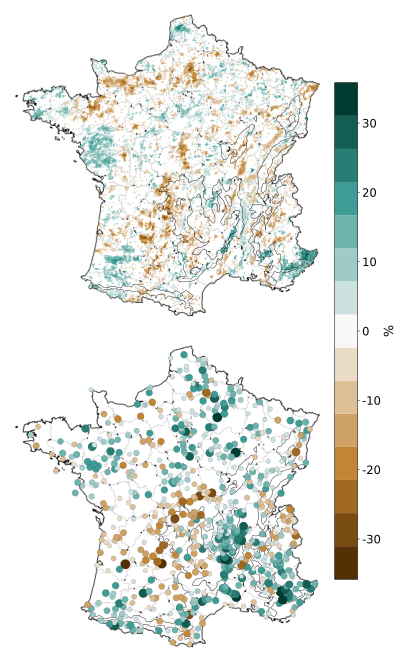
\includegraphics[width=\linewidth]{figures/trend_pluie_hydro.pdf} &
\begin{minipage}[c]{\linewidth}
  \centering
  \vspace{0.5em}
  \begin{minipage}[c]{0.90\linewidth}
    \setlength{\parindent}{0pt}
    \small
    \setcounter{figure}{4}% prochaine légende = Figure 5
    \captionof{figure}{
      \vspace{0.3em}
      Seasonal analysis of relative trends from 1995 to 2022 (\%) in the 10-year return level
      between the AROME model (left) and Météo-France stations (right), with the correlation ($r$),
      the number of stations compared (n), and the bias ($ME$) derived from daily precipitation maxima
      from 1959 to 2022.
      \vspace{0.3em}
    }
  \end{minipage}
\end{minipage}
\\

\end{tabularx}
\end{minipage}
\endgroup




\end{document}
